\section{Reconnaître des mélanges (2 points)}\label{ex:melanges}

\begin{center}
	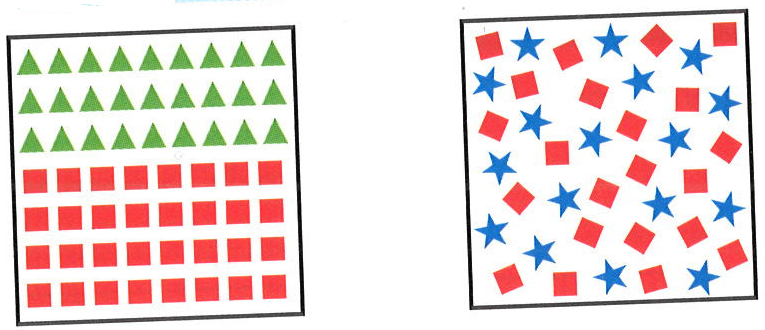
\includegraphics[scale=0.4]{img/melanges}
\end{center}

Ces schémas représentent deux mélanges différents.

\begin{questions}
	\question[1] Dans quel mélange est-il possible de distinguer les espèces chimiques mélangées ? Donner un exemple d'un tel mélange.
	
	\begin{solution}
		On fait clairement la distinction entre les deux espèces chimiques dans le premier mélange. C'est le cas lorsque l'on mélange de l'eau et de l'huile.
	\end{solution}
	
	\question[1] Dans quel mélange n'est-il pas possible de distinguer les espèces chimiques mélangées ? Donner un exemple d'un tel mélange.
	\begin{solution}
		On ne fait pas la distinction entre les deux espèces chimiques dans le second mélange. C'est le cas lorsque l'on mélange de l'eau et du sucre.
	\end{solution}
\end{questions}